\begin{frame}{Activation}

\begin{itemize}
    \item Just like Fully-Connected Neural Networks, we can apply an activation over convolutional layer outputs
    \item It helps break linearity
    \item For example, Rectified Linear Unit (ReLU): $\sigma(x) = max(0,x)$
\end{itemize}


\begin{figure}
\centering
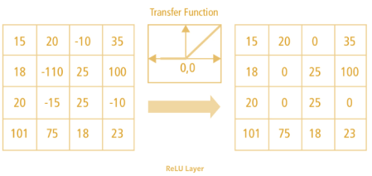
\includegraphics[width=1.0\textwidth,height=0.6\textheight,keepaspectratio]{images/cnn/activation.png}
\end{figure}

\end{frame}

\begin{frame}[fragile]{Activation Functions}
\begin{block}{Role:}
    \begin{itemize}
        \item Introduce non‑linearity so multiple conv layers can learn complex mappings.
    \end{itemize}
\end{block}

\begin{block}{Common:}
    \begin{itemize}
        \item ReLU (Rectified Linear Unit)
        \item Leaky ReLU
        \item Sigmoid
        \item Tanh
    \end{itemize}
\end{block}

\begin{lstlisting}[language=Python, caption={Code snippet (PyTorch)}, basicstyle=\ttfamily\footnotesize]
import torch.nn.functional as F

x = conv(input_tensor)
x = F.relu(x)              # ReLU
x = F.leaky_relu(x, 0.1)   # Leaky ReLU
\end{lstlisting}
\end{frame}  

\begin{frame}{Activation Functions}
    \begin{figure}
    \centering
    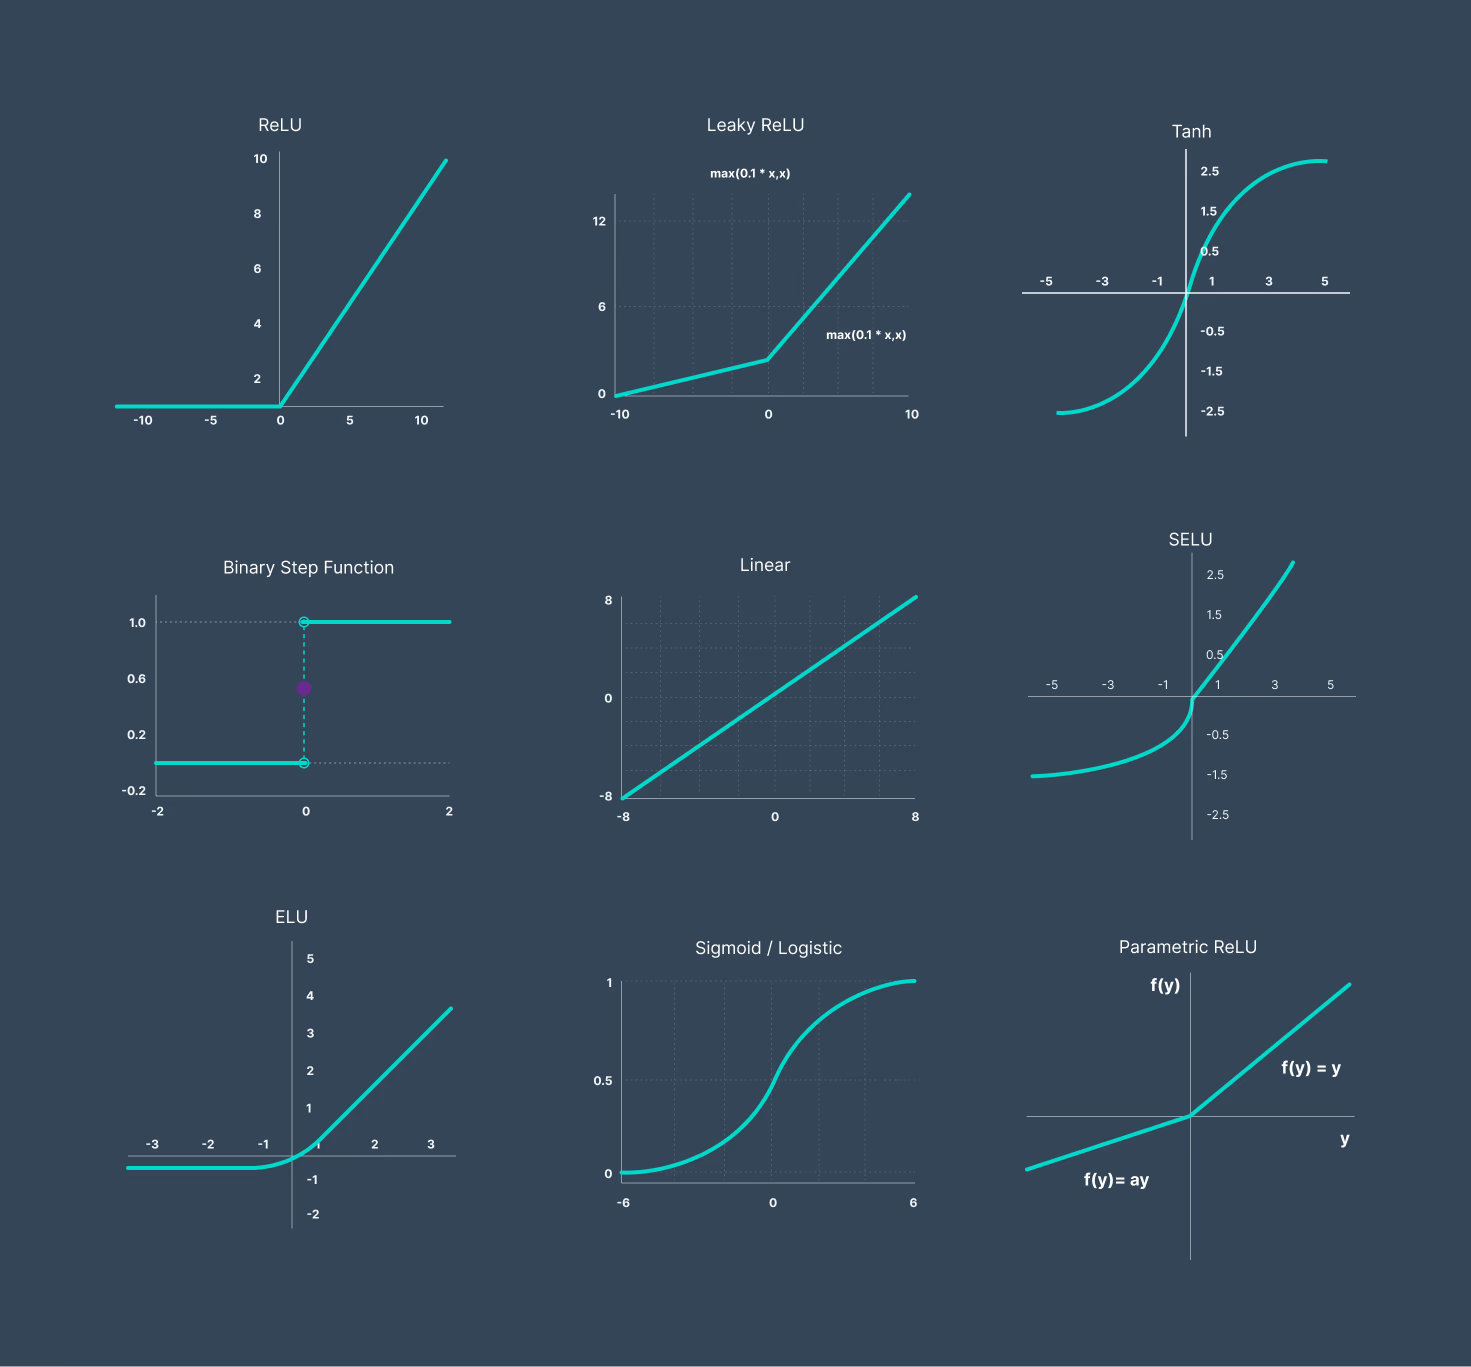
\includegraphics[width=0.95\textwidth,height=0.95\textheight,keepaspectratio]{images/cnn/activation-functions.png}
    \end{figure}
\end{frame}